% article example for classicthesis.sty
\documentclass[10pt,a4paper]{article} % KOMA-Script article scrartcl
\usepackage{import}
\usepackage{xifthen}
\usepackage{pdfpages}
\usepackage{transparent}
\newcommand{\incfig}[1]{%
    \def\svgwidth{\columnwidth}
    \import{./figures/}{#1.pdf_tex}
}
\usepackage{lipsum}     %lorem ipsum text
\usepackage{titlesec}   %Section settings
\usepackage{titling}    %Title settings
\usepackage[margin=10em]{geometry}  %Adjusting margins
\usepackage{setspace}
\usepackage{listings}
\usepackage{amsmath}    %Display equations options
\usepackage{amssymb}    %More symbols
\usepackage{xcolor}     %Color settings
\usepackage{pagecolor}
\usepackage{mdframed}
\usepackage[spanish]{babel}
\usepackage[utf8]{inputenc}
\usepackage{longtable}
\usepackage{multicol}
\usepackage{graphicx}
\graphicspath{ {./Images/} }
\setlength{\columnsep}{1cm}

% ====| color de la pagina y del fondo |==== %
\pagecolor{black}
\color{white}



\begin{document}
    %========================{TITLE}====================%
    \title{\rmfamily\normalfont\spacedallcaps{ Laboratorio 3:Forensics }}
    \author{\spacedlowsmallcaps{Rodrigo Castillo}}
    \date{\today}

    \maketitle


    %=======================NOTES GOES HERE===================%
    \section{Read the first paragraphs of the Section "Malware Analysis in
    Virtual Machines". Mention 1 advantage of using physical machines instead
    of virtual machines?}
        one of the advantages of using a physical machine is that it have full
        control of the resources of the machine, so it's faster.

    \section{Networking on VMs: Review the section "Configure Vmware".
    Regarding the networking configuration of a virtual machine, mention one
    advantage and one disadvantage of each possible networking configuration:}

        \subsection{Disconnected VM}
            \subsubsection{Advantages}
                One of the advantages of having your virtual machine
                disconnected is that a worm wont be able to spread over your
                network
            \subsubsection{Disadvantages}
                By the way, the machine wont be able to connect to internet,
                so, for example, if a malware need internet to work, the
                analysis wont enought.

        \subsection{Host-Only}
            \subsubsection{Advantages}
                Its usefull when you need to use internet in the virtual
                machine with the Ip of your real computer.
            \subsubsection{Disadvantages}
                malware can comunicate with host.

        \subsection{Multiple VMs inside an Internal Network}
            \subsubsection{Advantages}
                its usefull to analyze the way that malware spreads.
            \subsubsection{Disadvantages}
                the machines wont be able to communicate out to the internet.

        \subsection{VM with Bridged network adapter}
            \subsubsection{Advantages}
                It can be usefull to connect across the internet using an ip
                different to host.
            \subsubsection{Disadvantages}
                The malware can access to all machines in the network.

        \subsection{VM with NAT(Network Address Translation)}
            \subsubsection{Advantages}
               this mode is going to take the ip of the host machine.
            \subsubsection{Disadvantages}
                the malware can touch the host machine, also, internet is not
                safe, sometimes malware communicate with servers that are owned
                by mad people.

        \section{Wanna Cry}
        \color{red} i'm having problems with my virtual machine right now :( , so i
        think i'll have to execute this file later, by the way, i've runned a
        lot of ransomwares before in competitions \color{white}.
        \\ by the way, classic wannacry looks like this :
            \\
            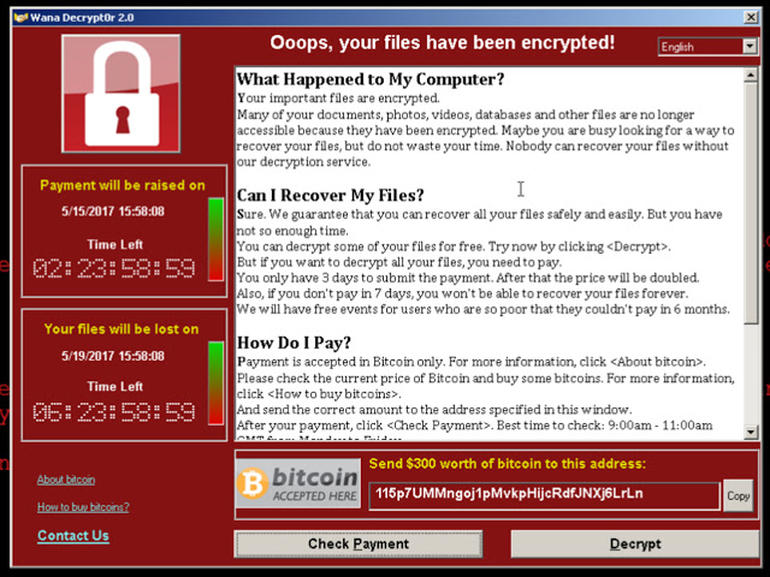
\includegraphics[width=0.8\linewidth]{wannacry.jpg}
            \\

        \section{Read the first paragraphs of the section "Basic Dynamic
        Analysis" and indicate one disadvantage of doing "dynamic analysis"
        without doing previously "static analysis".}
            Performig Basic Dynamic Analysis without performing static analysis
            before is just running malware blindly . When you are gonna analyze
            malware, at firts, you need to know which kind of malware are you
            going to analyze and how, then you can running for analyze the way
            it works.

        \section{Review the section "Sandboxes: The Quick-and-Dirty Approach".
        Then do the following steps over the malware "Redbear.exe" that you may
        download from here. Use the password: "forense" to decompress:}
        \color{red} because im having problem with my virtual machine, i cant
        use the tool PeID, so i'll use a similar tool called "Detect it easy"
        that works for linux .
        \\
        \color{white}
        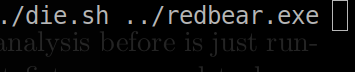
\includegraphics[width=0.4\linewidth]{diesh.png}
        \\
        from this tool, i can also check the memory of the malware, unfortunatly, even if the malware is obviusly packed, the tool just detects this:
        \\ 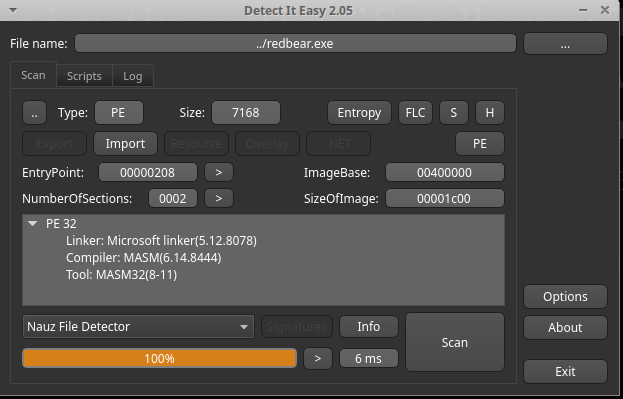
\includegraphics[width=0.8\linewidth]{compiler.png}
        \\
        i also checked the memory of the malware searching for packages, but it looks like this :
        \\ 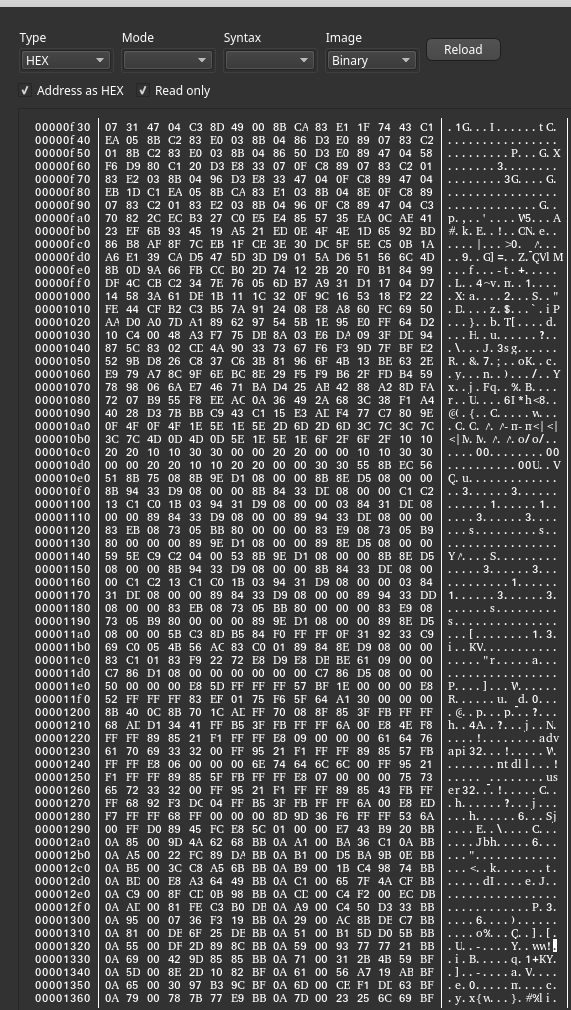
\includegraphics[width=0.8\linewidth]{memorydump.png}
        \\
        if you check for the entropy of the character of the malware, is obviusly packaged :
        \\ 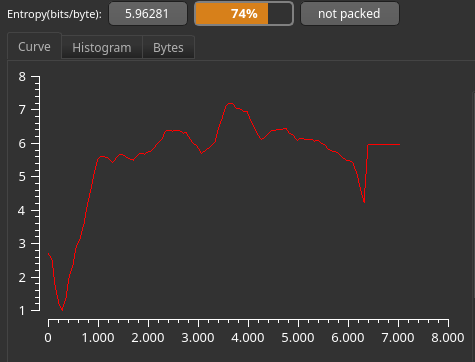
\includegraphics[width=0.8\linewidth]{compression_entropy.png}
        \\
        finally, i found a way to run PeID on linux, and i know that the
        malware is packed in a compression called junkcode
        \\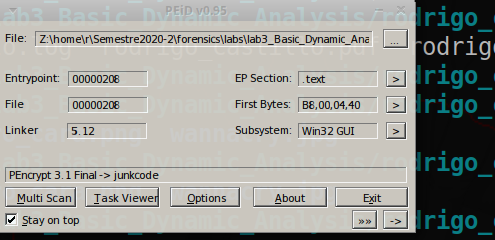
\includegraphics[width=0.8\linewidth]{packed.png}
        \\
        we can see that is a malware from " www.practicalmalwareanalysis.com" ,
        its a trojan that connects to this domain.Actually, we can see that is
        a reverse shell.\\
        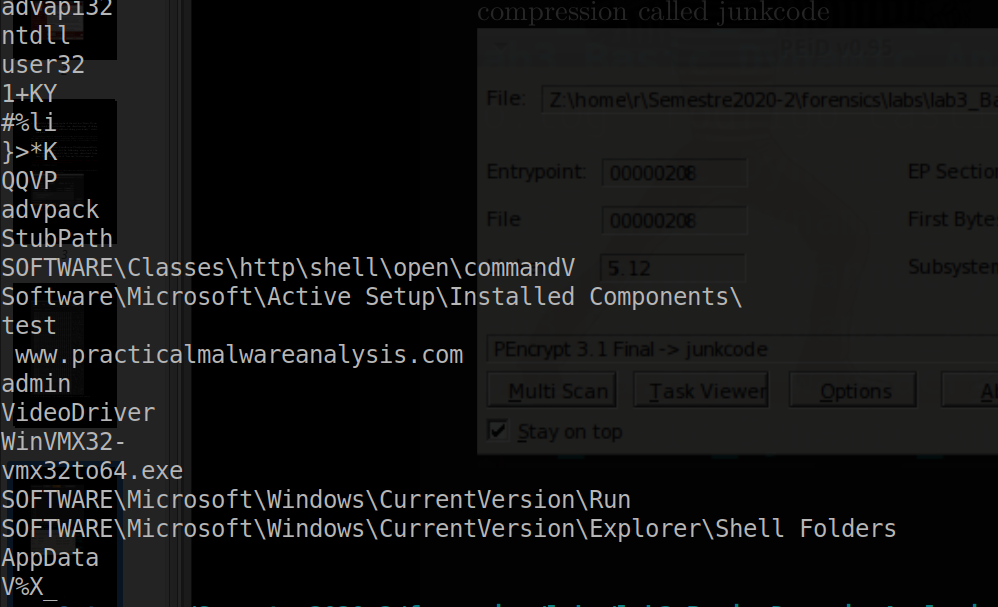
\includegraphics[width=0.8\linewidth]{strings.png}
        \\
        we also can see that it imports kernel32 library so its dangerous, in the binary we can see those paths :
        \\ 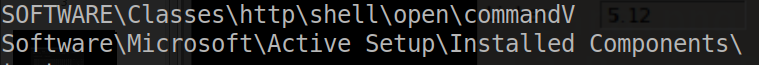
\includegraphics[width=0.5\linewidth]{newfiles.png}
        \\ i dont know too much about windows 32 architecture, but, those path
        can mean 2 things, the firstone is that he es creating this file for
        adding malware there, or the secondone is that the malware is modifying
        this file for addding malware there.

        \\ i checked that my analysis was ok in virus total and i was ok. Its a
        trojan for malware analysis.
        \\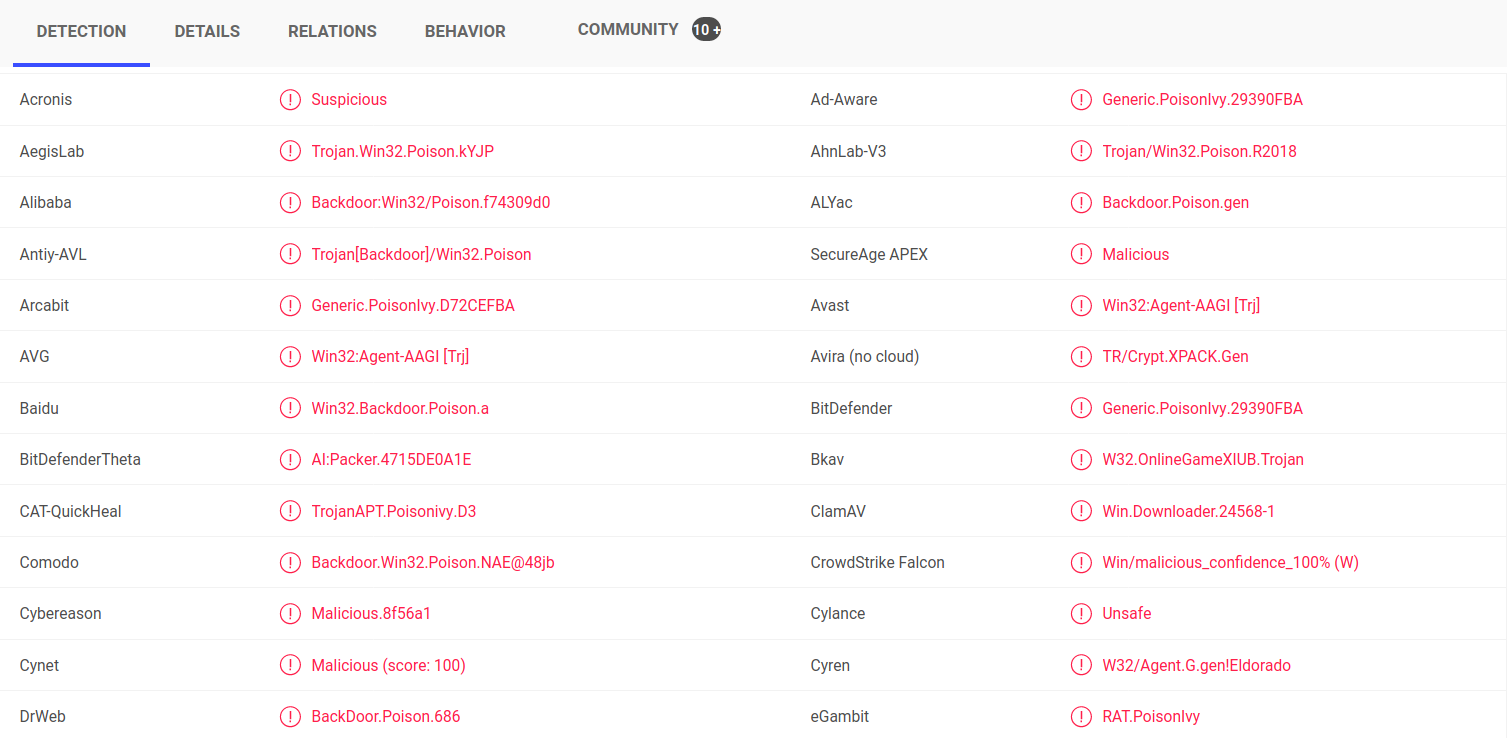
\includegraphics[width=0.8\linewidth]{trojan.png}
        \\
        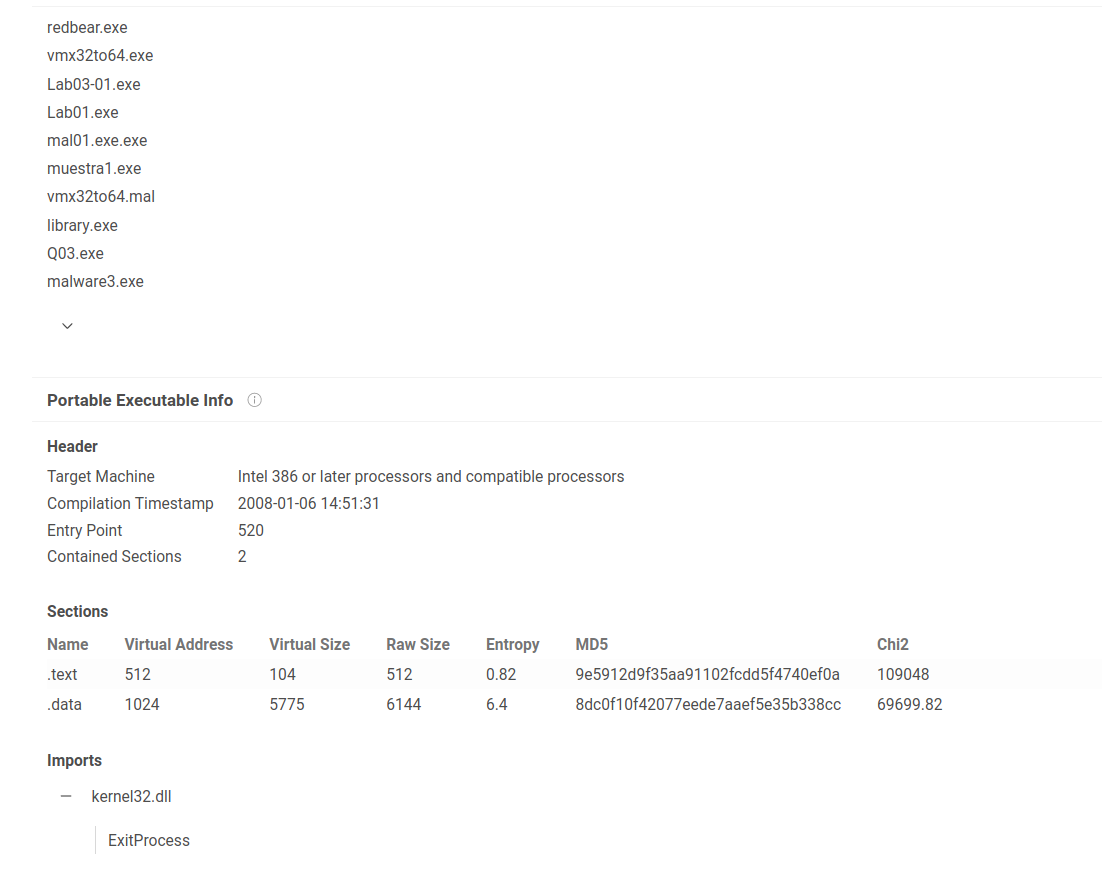
\includegraphics[width=0.8\linewidth]{names.png}
        \\






























    %=======================NOTES ENDS HERE===================%

    % bib stuff
    \nocite{*}
    \addtocontents{toc}{\protect\vspace{\beforebibskip}}
    \addcontentsline{toc}{section}{\refname}
    \bibliographystyle{plain}
    \bibliography{../Bibliography}
\end{document}
